%  CONFIGURE NEWcitep SINGLE-PAGE FORMAT

\onecolumn % go back to one column
%\fancyhead{} % make sure we get no headers
\renewcommand{\floatpagefraction}{0.1}
%\lfoot[\bSupInf]{\dAuthor}
%\rfoot[\dAuthor]{\cSupInf}
\newpage

%\captionsetup*{format=largeformat} % make figure legend slightly larger than in the paper
\setcounter{figure}{0} % reset figure counter for Supp. Figures
\setcounter{equation}{0} % reset equation counter for Supp. Equations
%\setcounter{page}{1} % reset page count
%\makeatletter
%\renewcommand{\thefigure}{S\@arabic\c@figure} % make Figure legend start with Figure S
%\makeatother
%\def\theequation{S\arabic{equation}}
\renewcommand{\figurename}{Supplementary Figure}

%  MAIN TEXT

\section*{Supplementary Information}
\newpage

%%%%%%%%%%%%%%%%%%%%%%%%%%%%%%%%%%%%%%%%%%%%%%%%%%%%%%%%%%%%%%%%%%%%%%%%%%%%%%%%
%
% Supp fig 1: Percent of explained loci
%
%%%%%%%%%%%%%%%%%%%%%%%%%%%%%%%%%%%%%%%%%%%%%%%%%%%%%%%%%%%%%%%%%%%%%%%%%%%%%%%%

%\begin{figure}[!tbp]
%    \centering
%    \includegraphics[width=\textwidth]{\floatRelativePath/cmpt_perc_tophits_eqtl.py/subplots.png}
%
%    \caption{}
%%
%\end{figure}

%%%%%%%%%%%%%%%%%%%%%%%%%%%%%%%%%%%%%%%%%%%%%%%%%%%%%%%%%%%%%%%%%%%%%%%%%%%%%%%%
%
% Fig 2: ucsc screenshots
%
%%%%%%%%%%%%%%%%%%%%%%%%%%%%%%%%%%%%%%%%%%%%%%%%%%%%%%%%%%%%%%%%%%%%%%%%%%%%%%%%

%\begin{figure}[!ht]
%    \centering
\rotatebox{90}{
\begin{minipage}{1.6\textwidth}

%    \begin{subfigure}[]{\textwidth}
%    https://genome-euro.ucsc.edu/cgi-bin/hgTracks?db=hg38&lastVirtModeType=default&lastVirtModeExtraState=&virtModeType=default&virtMode=0&nonVirtPosition=&position=chr5%3A132217324%2D132511091&hgsid=304633938_J4NJ6AxL9TTbYQJWKp7GHbB1fiia
        \textbf{Supplementary Figure 1a}
        \\
        \includegraphics[width=\textwidth]{fig/ucsc_gwas2eqtl_bcell_chr5_132217324_132511091_help.drawio.png}
%    \end{subfigure}

%    \begin{subfigure}[]{0.99\textwidth}
%        \textbf{b}
%        \\
%        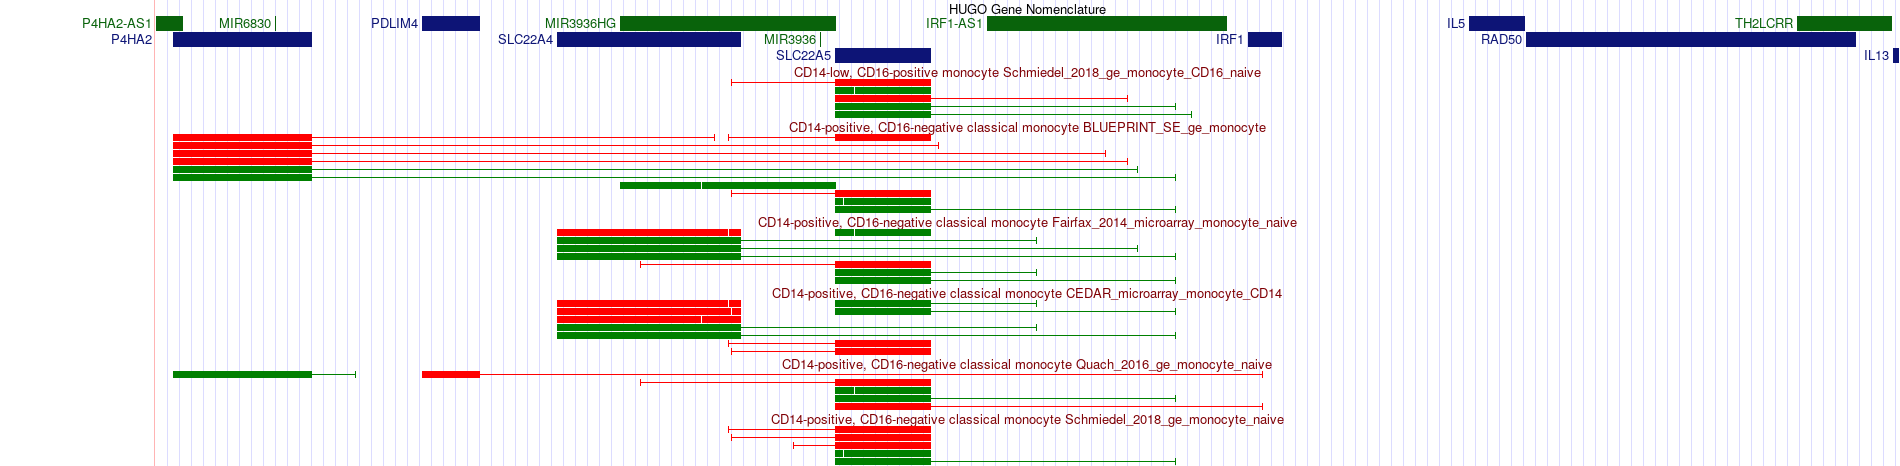
\includegraphics[width=\textwidth]{fig/ucsc_gwas2eqtl_il4_monocyte.png}
%    \end{subfigure}
%
%    \begin{subfigure}[]{0.99\textwidth}
%        \textbf{c}
%        \\
%        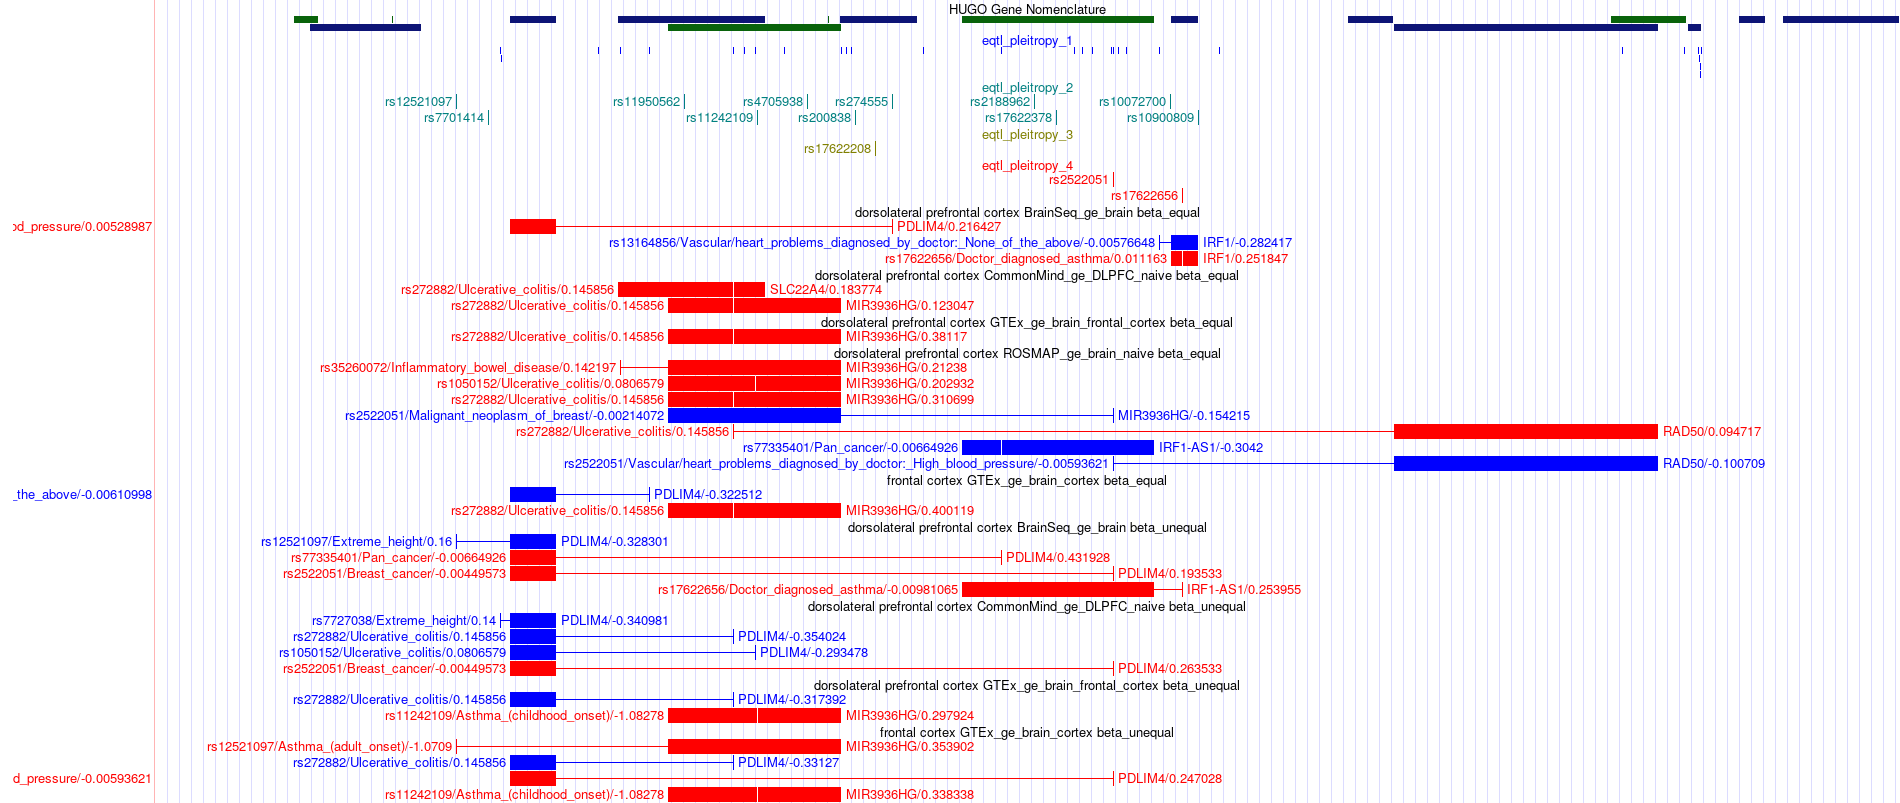
\includegraphics[width=\textwidth]{fig/ucsc_gwas2eqtl_il4_frontalcortex.png}
%    \end{subfigure}

%    \caption{}
\end{minipage}
}

%\end{figure}

%\begin{figure}[!ht]
%    \centering

\centering
\rotatebox{90}{
\begin{minipage}{1.4\textwidth}

%    \begin{subfigure}[]{\textwidth}
%        \textbf{a}
%        \\
%        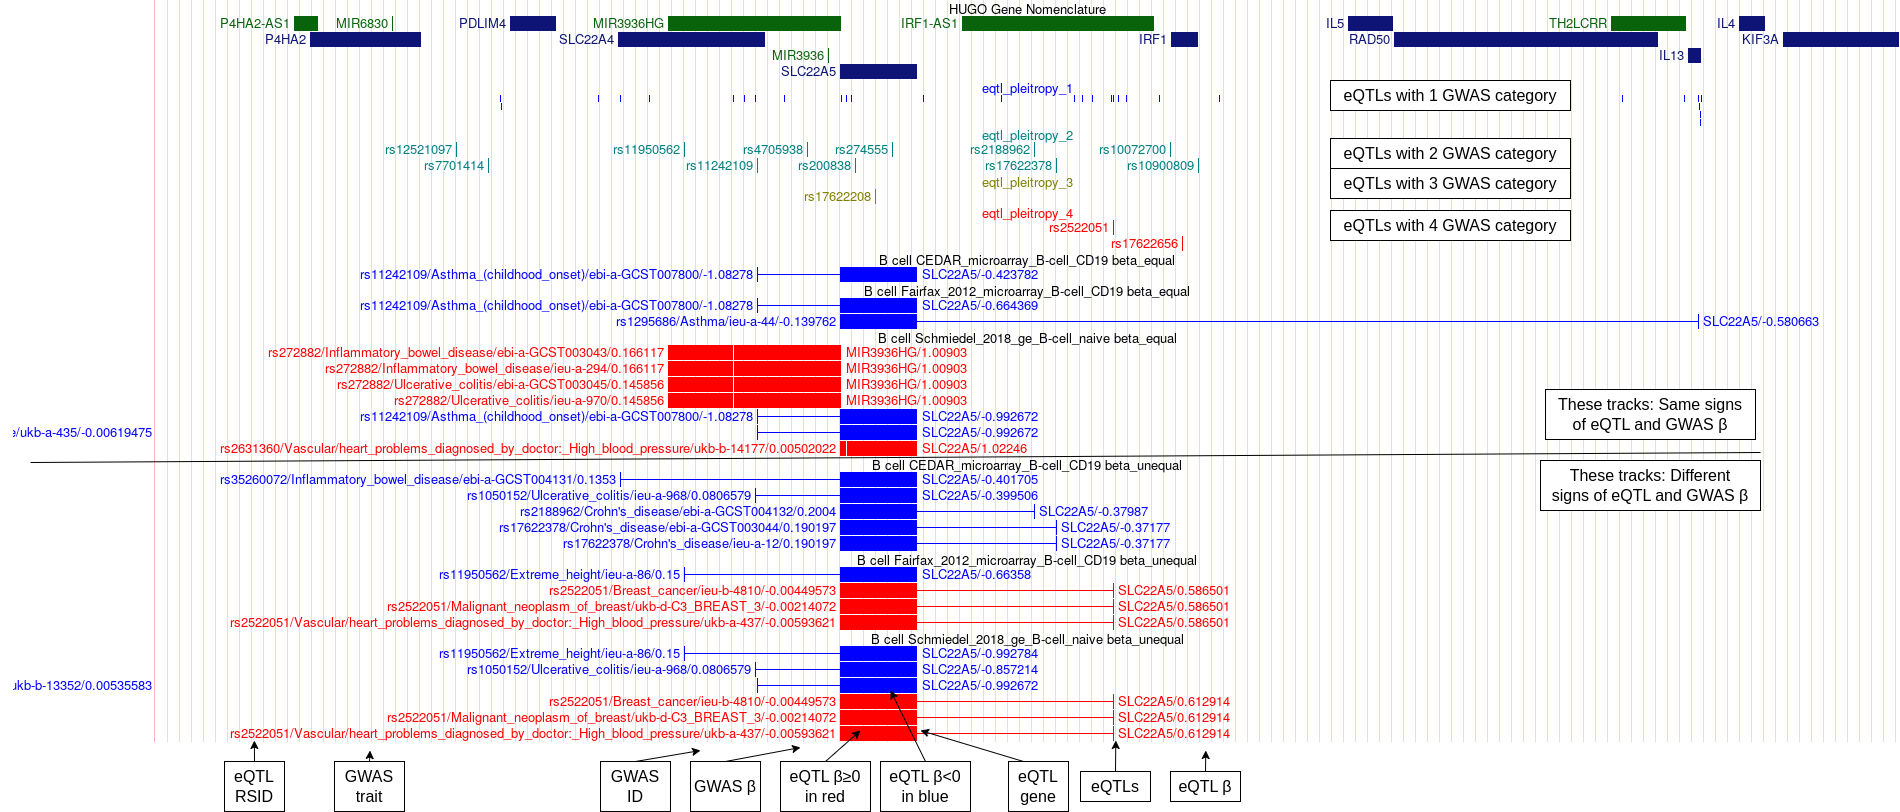
\includegraphics[width=\textwidth]{fig/ucsc_gwas2eqtl_il4_bcell_help.png}
%    \end{subfigure}

%    \begin{subfigure}[]{0.99\textwidth}
%    https://genome-euro.ucsc.edu/cgi-bin/hgTracks?db=hg38&lastVirtModeType=default&lastVirtModeExtraState=&virtModeType=default&virtMode=0&nonVirtPosition=&position=chr5%3A132102721%2D132543372&hgsid=304633938_J4NJ6AxL9TTbYQJWKp7GHbB1fiia
        \textbf{Supplementary Figure 1b}
        \\
        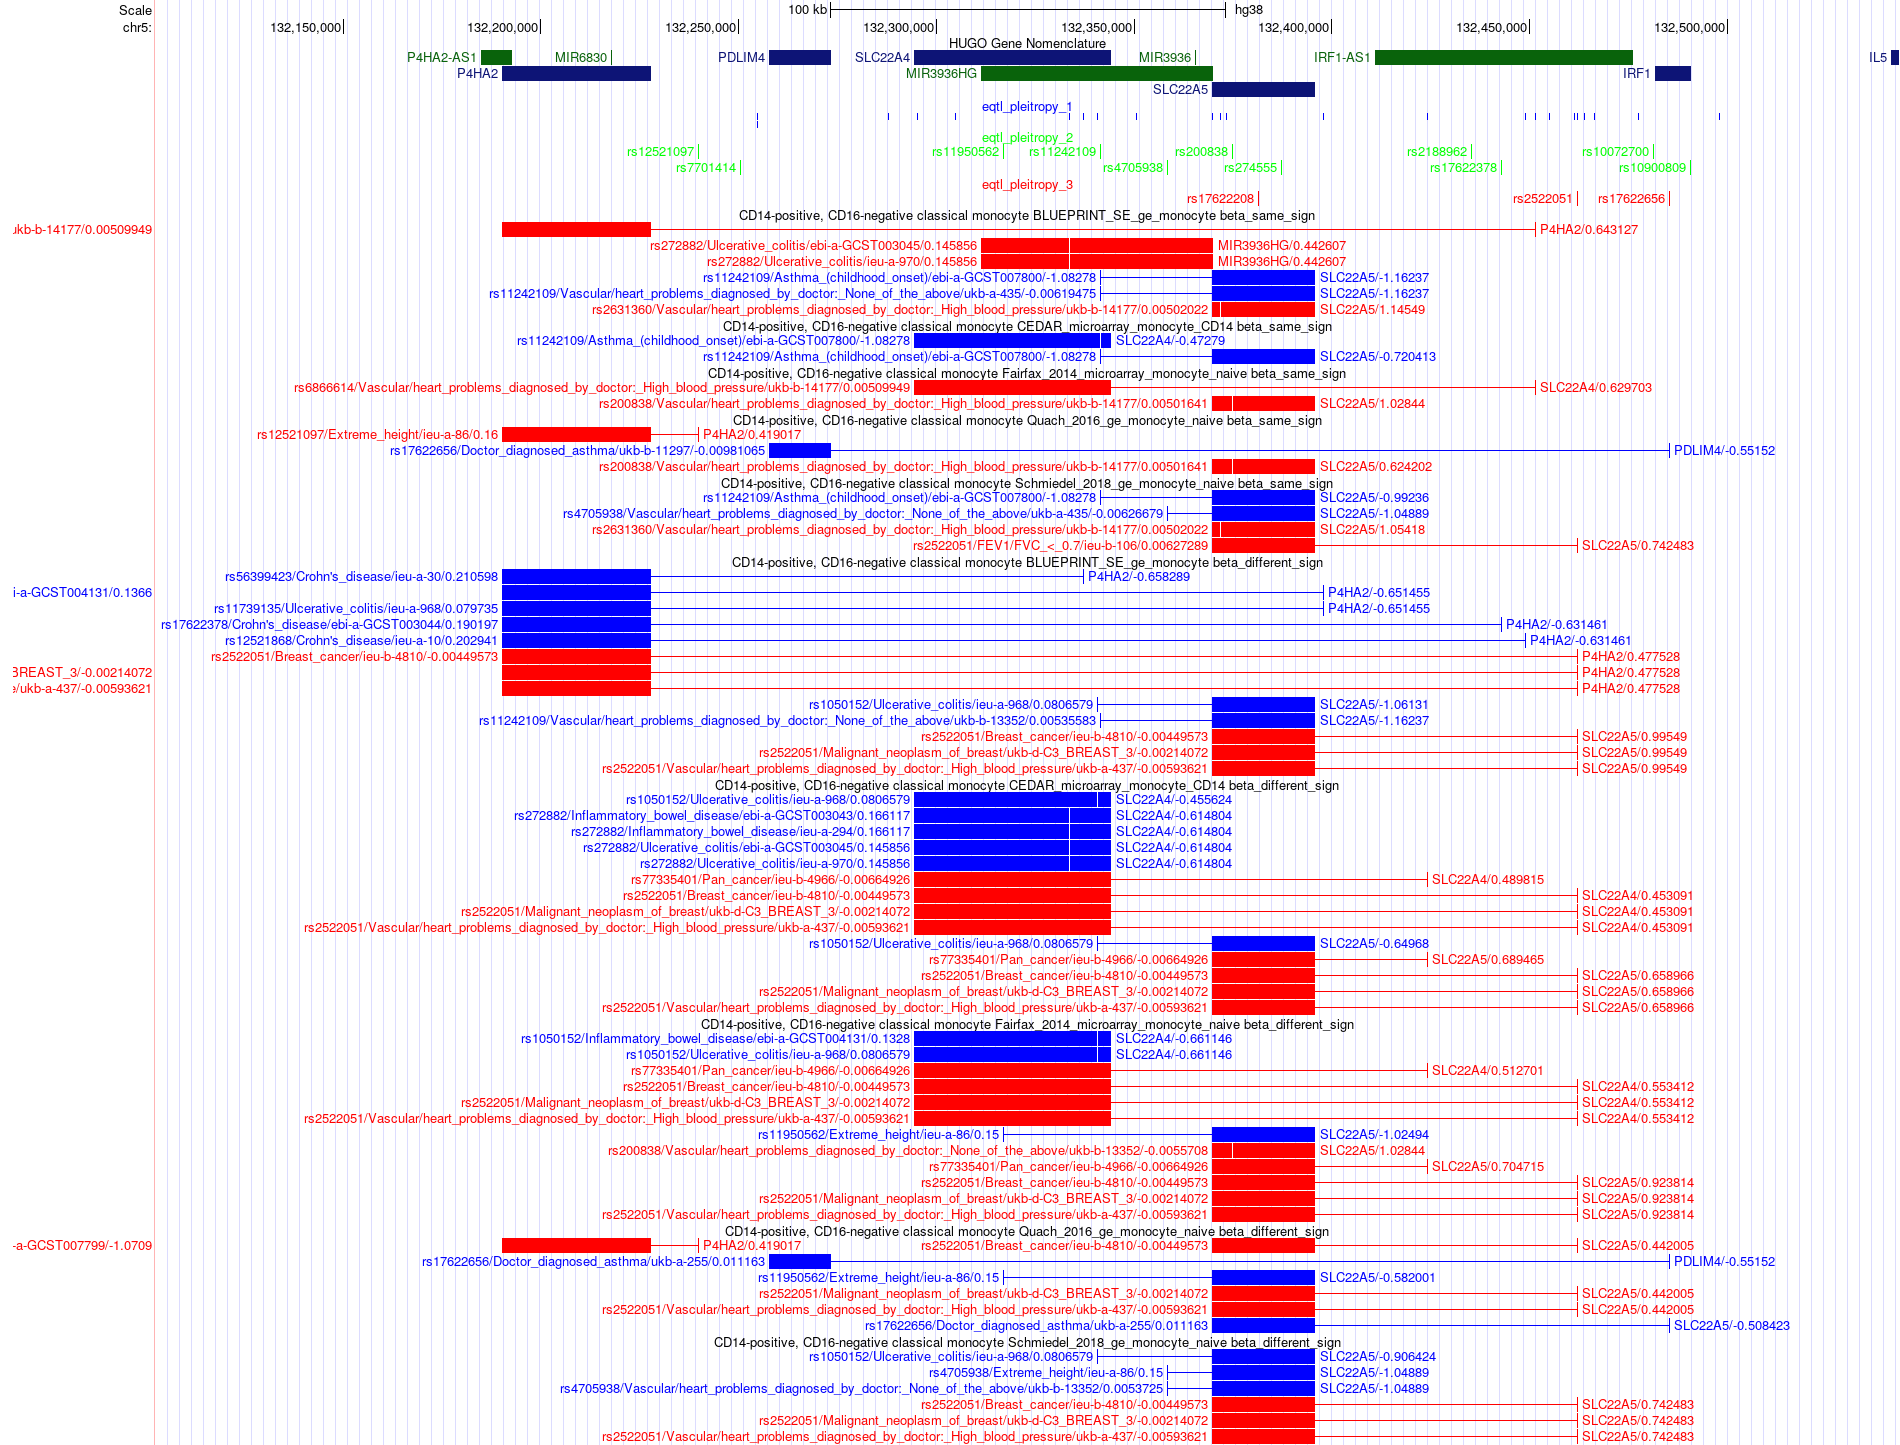
\includegraphics[width=\textwidth]{fig/ucsc_gwas2eqtl_monocyte_chr5_132102721_132543372.png}
%    \end{subfigure}
%
%    \begin{subfigure}[]{0.99\textwidth}
%        \textbf{c}
%        \\
%        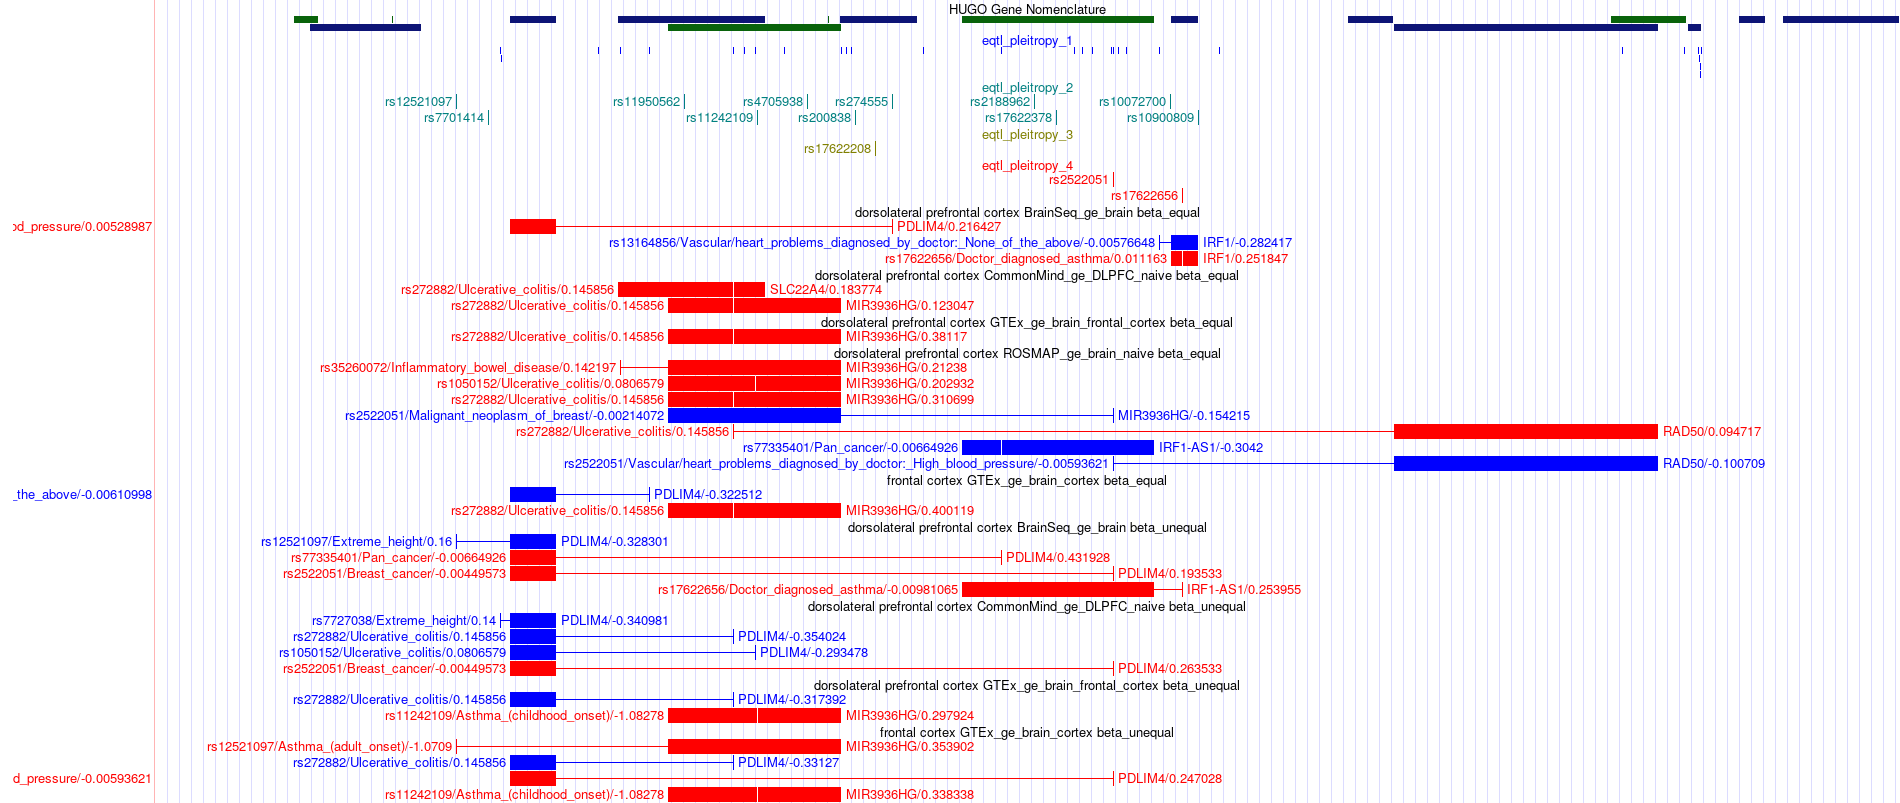
\includegraphics[width=\textwidth]{fig/ucsc_gwas2eqtl_il4_frontalcortex.png}
%    \end{subfigure}

%    \caption{}
\end{minipage}
}

%\end{figure}

%\begin{figure}[!ht]
%    \centering
\rotatebox{90}{
\begin{minipage}{1.6\textwidth}

%    \begin{subfigure}[]{\textwidth}
%        \textbf{a}
%        \\
%        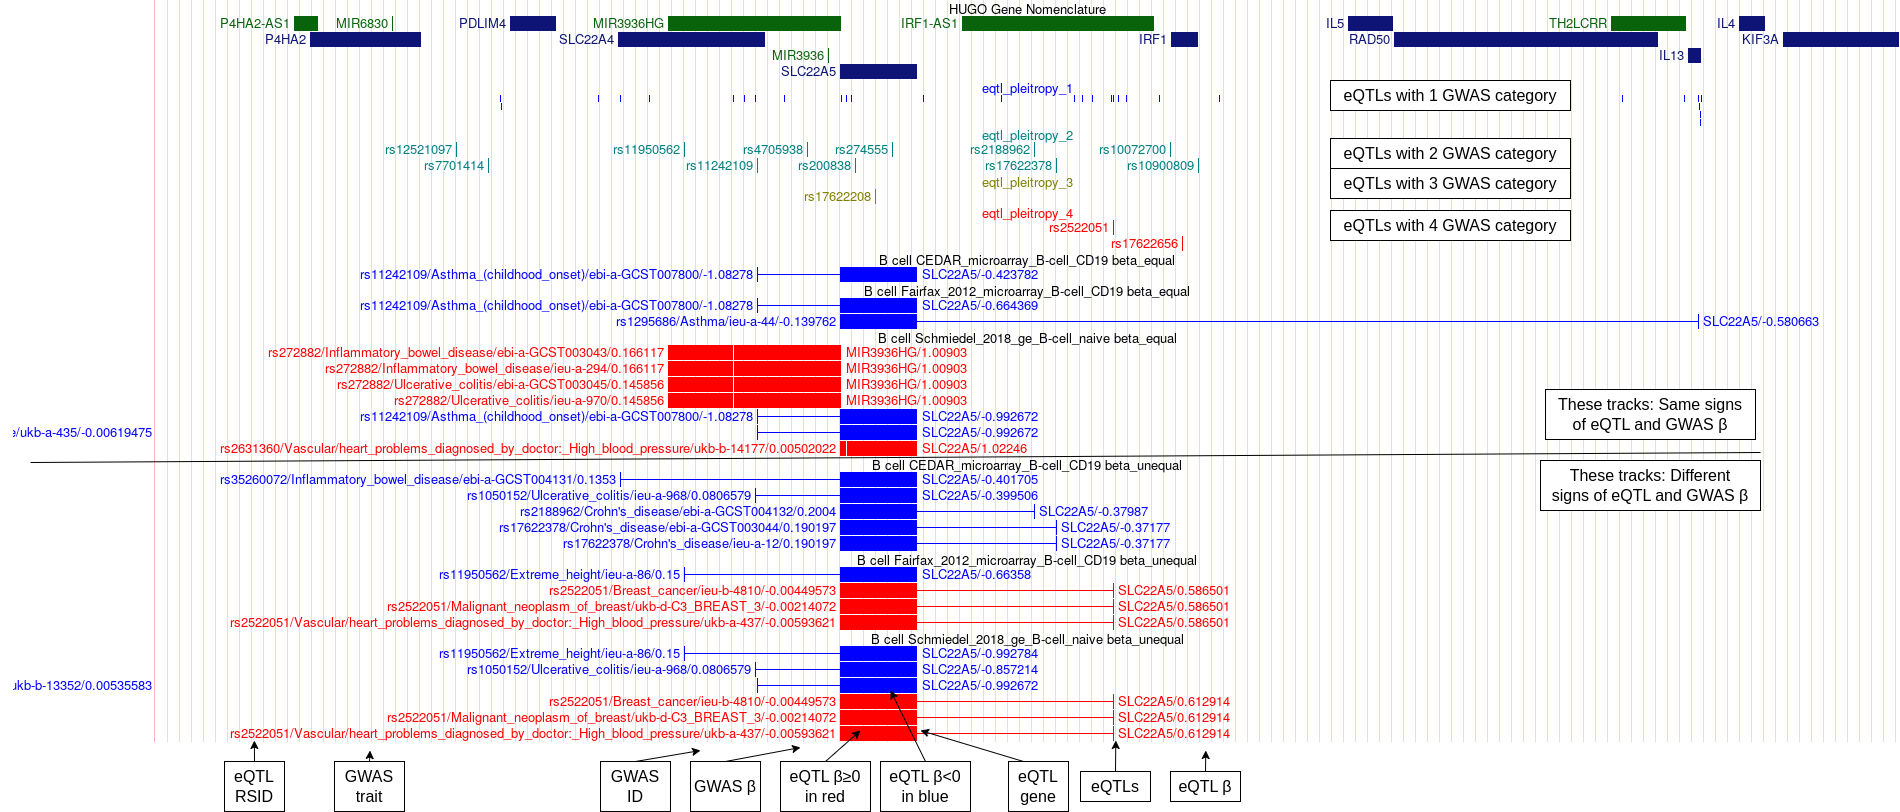
\includegraphics[width=\textwidth]{fig/ucsc_gwas2eqtl_il4_bcell_help.png}
%    \end{subfigure}

%    \begin{subfigure}[]{0.99\textwidth}
%        \textbf{b}
%        \\
%        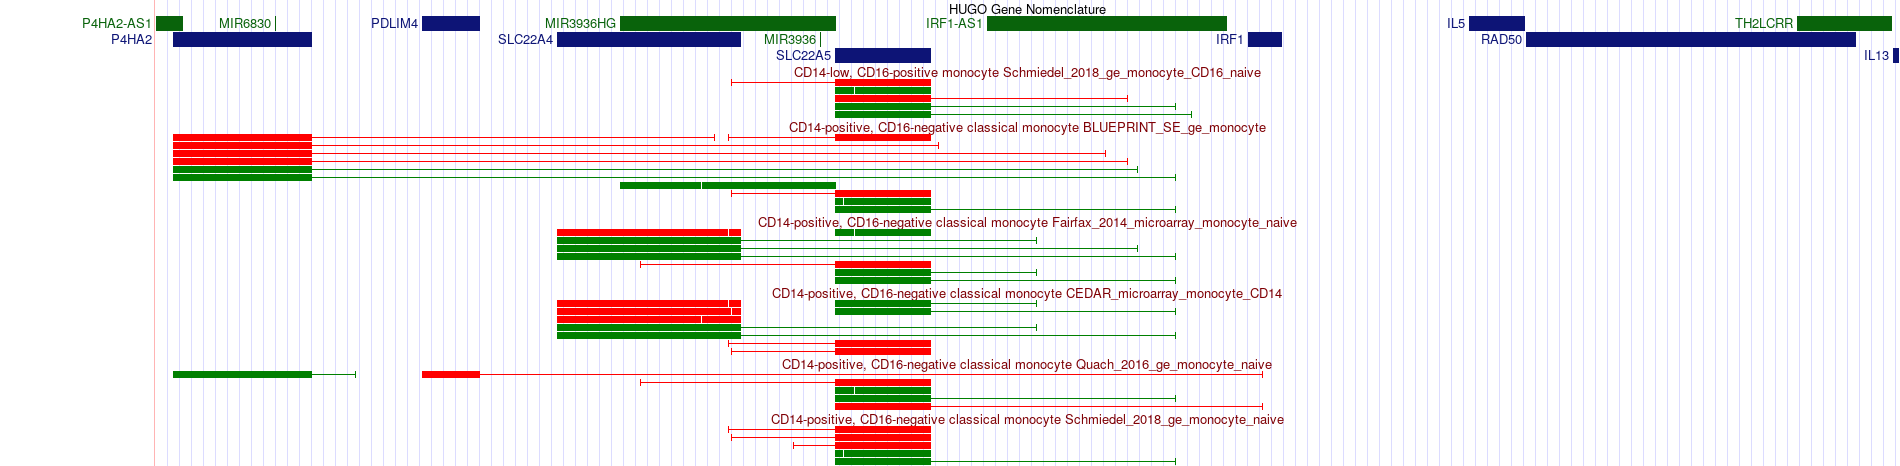
\includegraphics[width=\textwidth]{fig/ucsc_gwas2eqtl_il4_monocyte.png}
%    \end{subfigure}
%
%    \begin{subfigure}[]{0.99\textwidth}
        \textbf{Supplementary Figure 1c}
        \\
        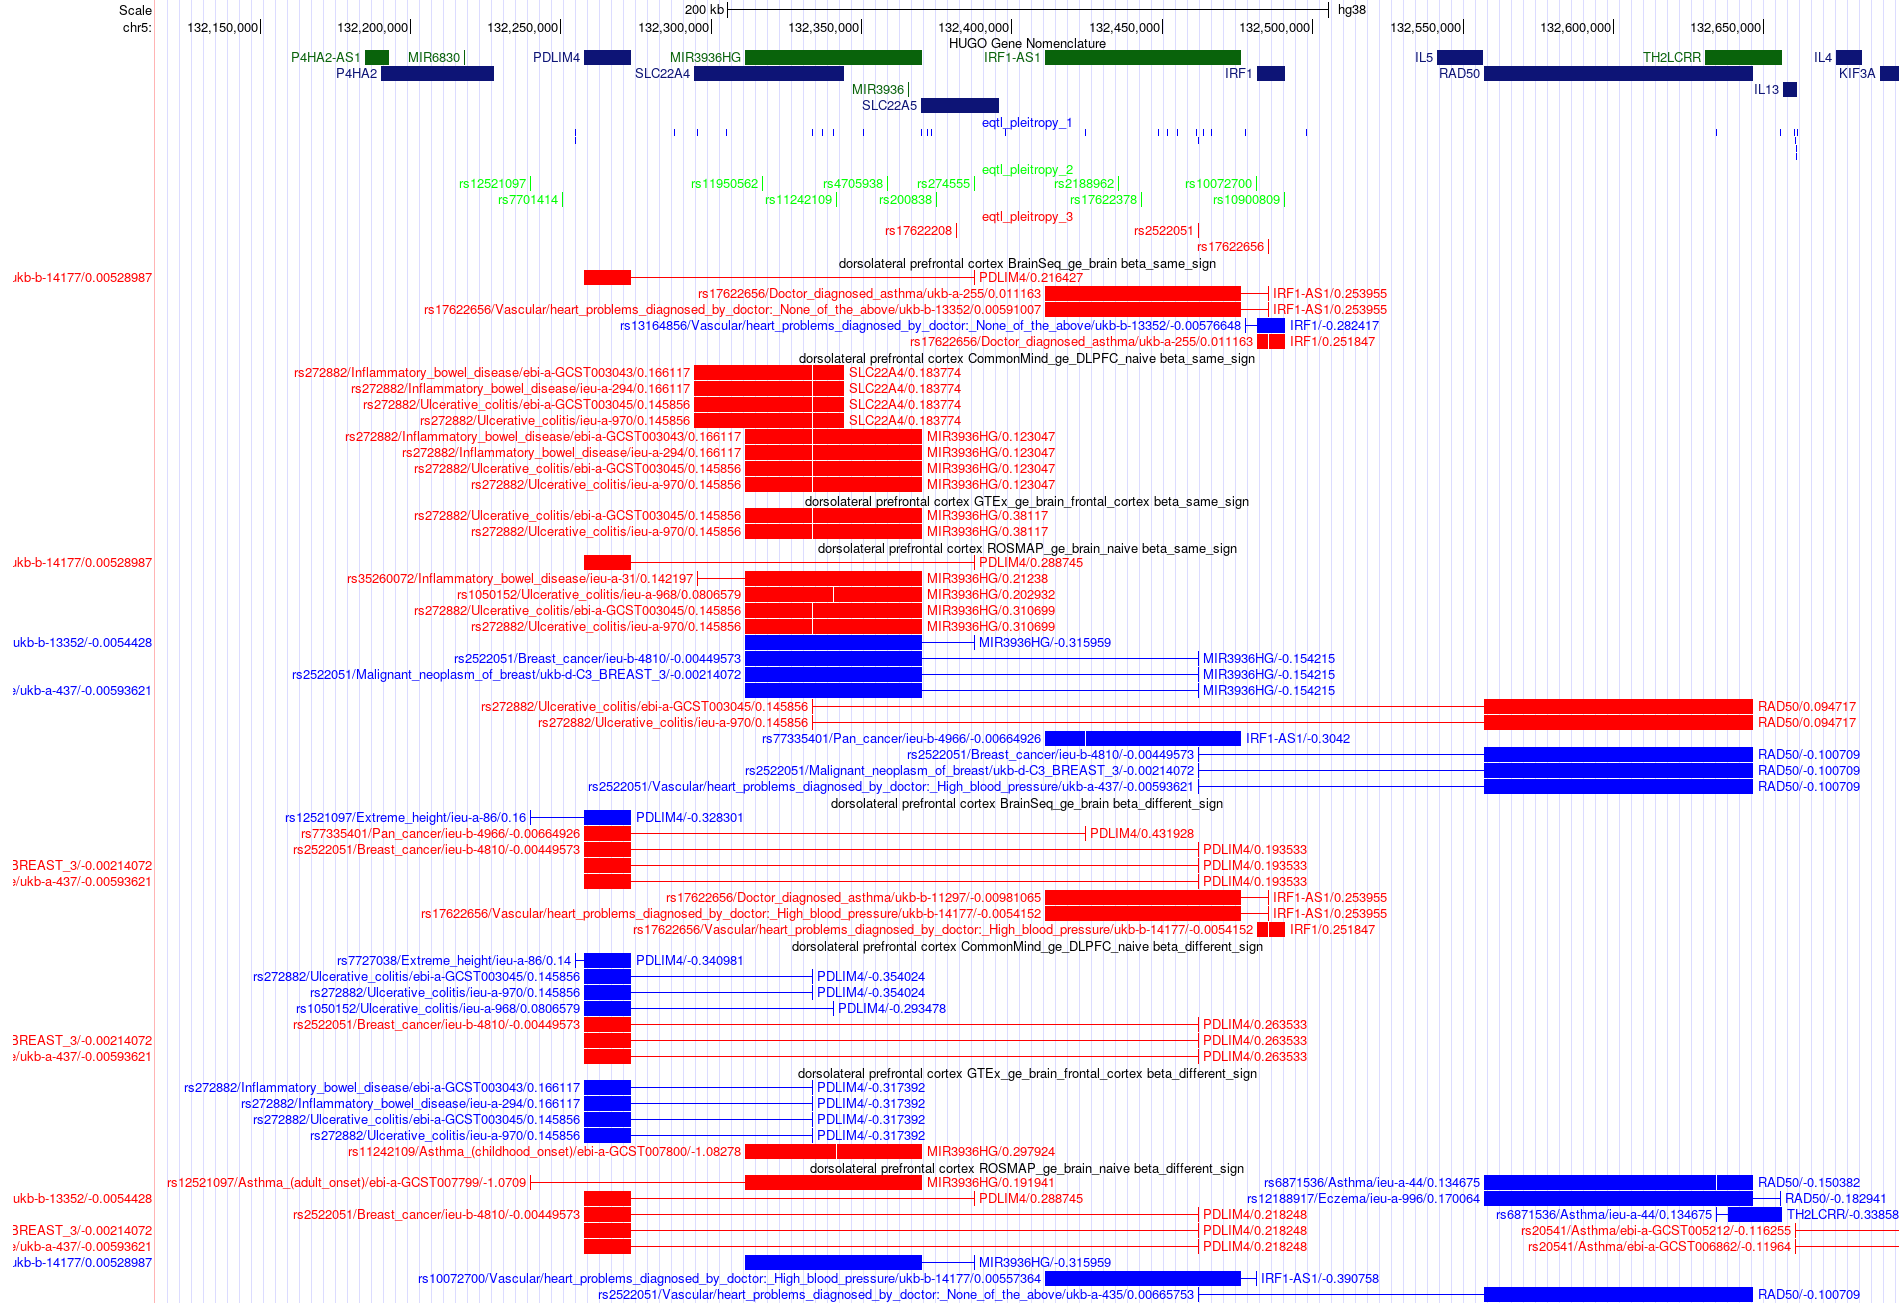
\includegraphics[width=\textwidth]{fig/ucsc_gwas2eqtl_frontalcortex_chr5_132115326_132695000.png}
%    \end{subfigure}

%    \caption{}
\end{minipage}
}

%\end{figure}

%%%%%%%%%%%%%%%%%%%%%%%%%%%%%%%%%%%%%%%%%%%%%%%%%%%%%%%%%%%%%%%%%%%%%%%%%%%%%%%%
%
% Fig 5: Comparison with Watanabe 2019
%
%%%%%%%%%%%%%%%%%%%%%%%%%%%%%%%%%%%%%%%%%%%%%%%%%%%%%%%%%%%%%%%%%%%%%%%%%%%%%%%%

\begin{figure}[!ht]
    %
    \centering
    %
    \begin{subfigure}[]{.49\textwidth}
        \textbf{a}
        \\
        \includegraphics[width=\textwidth]{\floatRelativePath/cmpt_count_per_rsid.py/watanabe_cat_count.png}
    \end{subfigure}
    %
    \begin{subfigure}[]{.49\textwidth}
        \textbf{b}
        \\
        \includegraphics[width=\textwidth]{\floatRelativePath/cmpt_count_per_rsid.py/watanabe_percentage.png}
    \end{subfigure}

    \caption{}

\end{figure}

%%%%%%%%%%%%%%%%%%%%%%%%%%%%%%%%%%%%%%%%%%%%%%%%%%%%%%%%%%%%%%%%%%%%%%%%%%%%%%%%
%
% Supp fig: allele frequencies
%
%%%%%%%%%%%%%%%%%%%%%%%%%%%%%%%%%%%%%%%%%%%%%%%%%%%%%%%%%%%%%%%%%%%%%%%%%%%%%%%%

\begin{figure}[!tbp]

    \begin{subfigure}[]{.49\textwidth}
        \textbf{a}
        \\
        \includegraphics[width=\textwidth]{\floatRelativePath/plt_x_per_variant_y_allele_freq.py/afr_af_custom.png}
    \end{subfigure}
%
    \begin{subfigure}[]{.49\textwidth}
        \textbf{b}
        \\
        \includegraphics[width=\textwidth]{\floatRelativePath/plt_x_per_variant_y_allele_freq.py/amr_af_custom.png}
    \end{subfigure}

    \begin{subfigure}[]{.49\textwidth}
        \textbf{c}
        \\
        \includegraphics[width=\textwidth]{\floatRelativePath/plt_x_per_variant_y_allele_freq.py/eas_af_custom.png}
    \end{subfigure}
%
    \centering
    \begin{subfigure}[]{.49\textwidth}
        \textbf{d}
        \\
        \includegraphics[width=\textwidth]{\floatRelativePath/plt_x_per_variant_y_allele_freq.py/sas_af_custom.png}
    \end{subfigure}

    \caption{}

\end{figure}


% Fig 9: eQTL gene distance furthest
\begin{figure}[!ht]
    \centering
    \begin{subfigure}[]{.49\textwidth}
        \includegraphics[width=\textwidth]{\floatRelativePath/plt_x_per_variant_y_egene_distance.py/boxenplot_custom_furthest_distance.png}
    \end{subfigure}

    \caption{}

\end{figure}


\begin{figure}[!ht]
    \centering
    \begin{subfigure}[]{.49\textwidth}
        \includegraphics[width=\textwidth]{\floatRelativePath/plt_x_per_variant_egene_y_etissue.py/plt.png}
    \end{subfigure}

    \caption{}

\end{figure}



